
\documentclass{beamer}
\mode<presentation> {
\usetheme{Singapore}
}

\usepackage{multicol}
\usepackage[russian]{babel}
\usepackage{graphicx} 
\usepackage{booktabs}


\title[Python Intro]{Introduction to Python} 

\author{Sugarkhuu Radnaa}
\institute[] 
{
Py4Econ in Ulaanbaatar \\
\medskip
\textit{py4econ@gmail.com} 
}
\date{}  

\begin{document}

\begin{frame}
\titlepage 
\end{frame}


% Notes
% All say hi
% Recording will start, then will be shared
% Facebook group chat
% My background 


\begin{frame}
\frametitle{About the course} 
\begin{enumerate}
    \item Basic programming know-hows
    \item Elementary to Intermediate Python
        \begin{itemize}
            \item Introductory section topics:
            \begin{itemize}
                \item Python specific:  Data basics, Functions/Class, Some useful knowledge
                \item General programming: Code editor (VScode), Git/Github
            \end{itemize}            
            \item Applications topics: Visualizaiton, Automation, Webscraping, ML/DL
        \end{itemize}
    \item Homework after each session
\end{enumerate}

\end{frame}

\begin{frame}
    \frametitle{About the course} % Table of contents slide, comment this block out to remove it
    \begin{itemize}
        \item To make the best out of the course:
            \begin{itemize}
                \item Submit homeworks in timely manner!
                \item Ask questions!
            \end{itemize}
    \end{itemize}        
    % \tableofcontents % Throughout your presentation, if you choose to use \section{} and \subsection{} commands, these will automatically be printed on this slide as an overview of your presentation
\end{frame}

\begin{frame}
    \frametitle{Week 1: Learning objectives}
    \begin{enumerate}
        \item Background information
        \item Python /Anaconda/
        \item VScode, Jupyter notebook and other IDEs
        \item Git \& Github
        \item Computer basics (Folder structures, Path, Shell)
    \end{enumerate}
\end{frame}


%------------------------------------------------
\section{Background information} 
% \begin{frame}
%     \tableofcontents[currentsection]
% \end{frame}
%------------------------------------------------



\begin{frame}
    \frametitle{Why Python?}
    \centering
    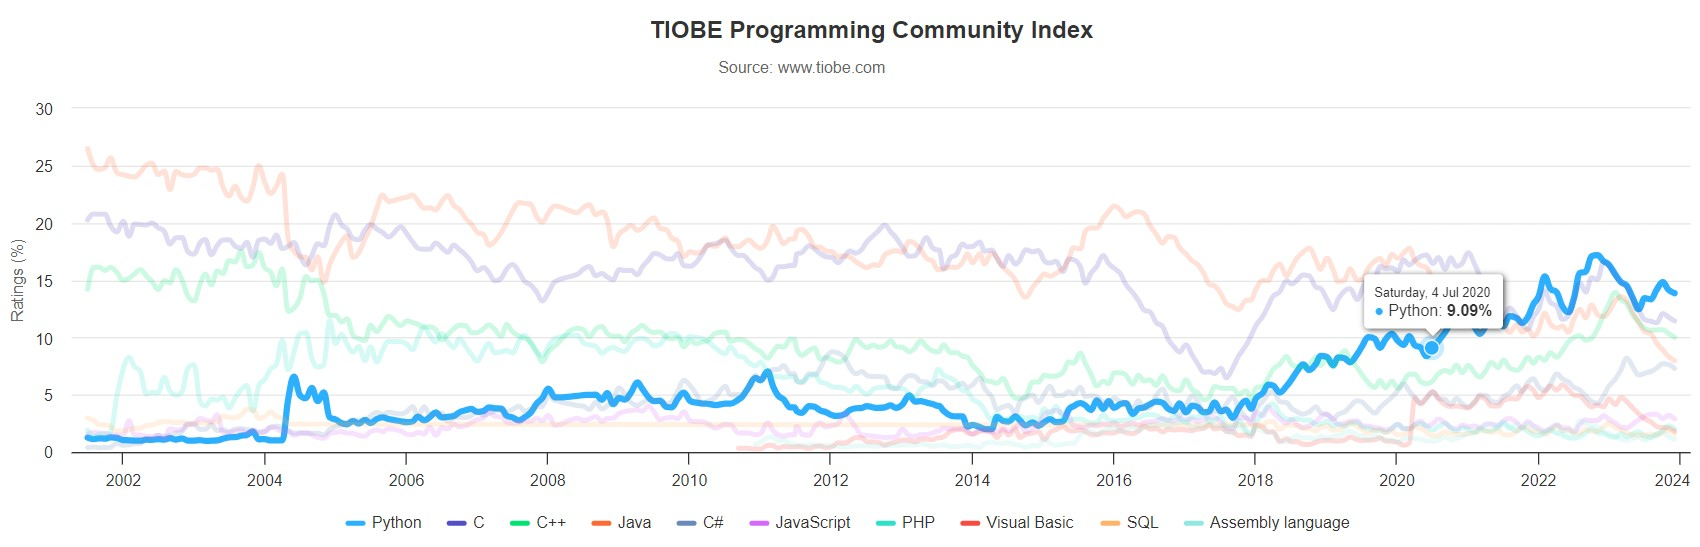
\includegraphics[scale = 0.3]{figures/trend_python.jpg}
\end{frame}

\begin{frame}
    \frametitle{Popular applications of Python}
    \begin{enumerate}
        \item Data science and data visualization
        \item Machine learning \& AI
        \item Scientific computing (incl. Financial modelling)
        \item Web \& Game development
        \item Desktop applications \& Software \& GUI
        \item Automation
    \end{enumerate}
\end{frame}

\begin{frame}
    \frametitle{Python was first released in 1991}
    \centering
    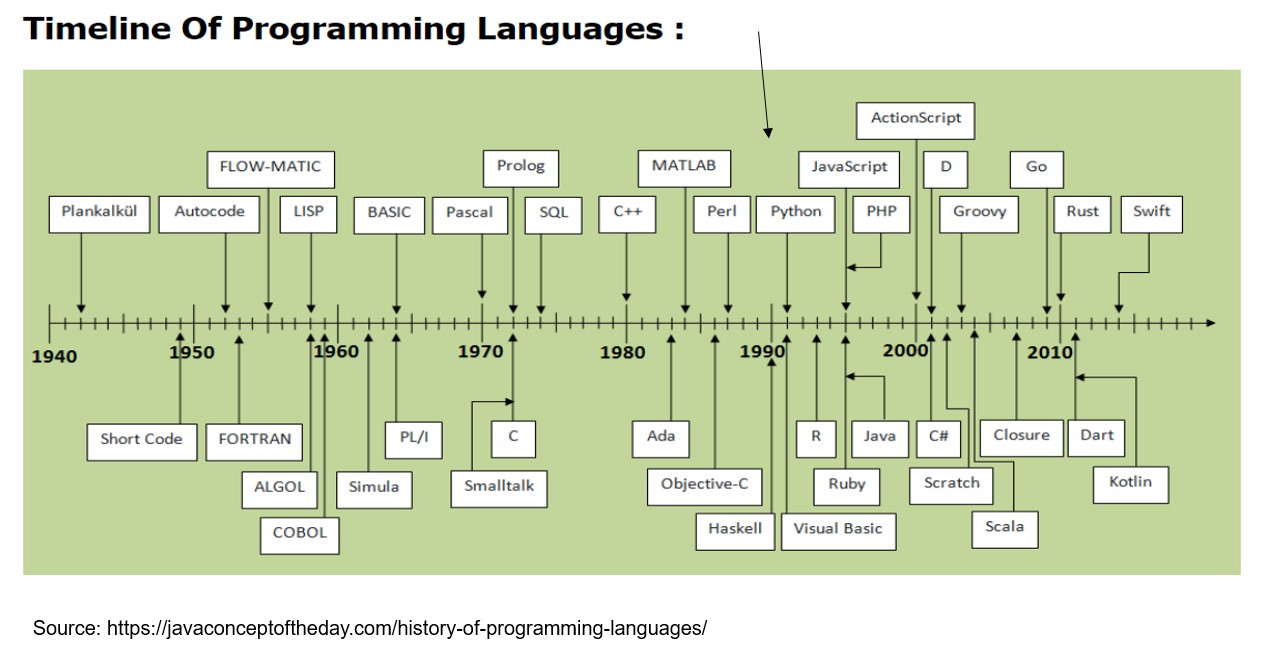
\includegraphics[scale = 0.4]{figures/timeline_lang.jpg}
\end{frame}

\begin{frame}
    \frametitle{Communities and learning platforms}
    \begin{multicols}{2}
        \begin{enumerate}
            \item Python - Official
            \item Stack overflow - Forum
            \item Medium - Blog
            \item Towardsdatascience - Blog
            \item Tutorialspoint
            \item Geek for geeks
            \item W3schools
            \item Real Python
            \item Programiz
            \item Kaggle - Competition and Learning resource
        \end{enumerate}
    \end{multicols}
\end{frame}

\begin{frame}
    \frametitle{Guide: Must-have basics for a good programmer}
    \begin{itemize}
        \item Data Structure and Algorithm
        \item A Version Control Tool (Git)
        \item One Text Editors (VScode)
        \item IDEs (Spyder or Pycharm)
        \item Database and SQL
        \item UNIX (Linux)
        \item An OOP Programming language (C++, Java or Python)
        \item One Scripting language (automation)
        \item Networking basics
        \item \textit{Cloud Platform (AWS, GCP, or Azure)}
        \item \textit{Containers (Docker and Kubernetes)}
    \end{itemize}
\end{frame}

%------------------------------------------------
\section{Computer basics and more} 
% \frame{\tableofcontents[currentsection]}
%------------------------------------------------

\begin{frame}
    \frametitle{Computer basics}
    \centering
    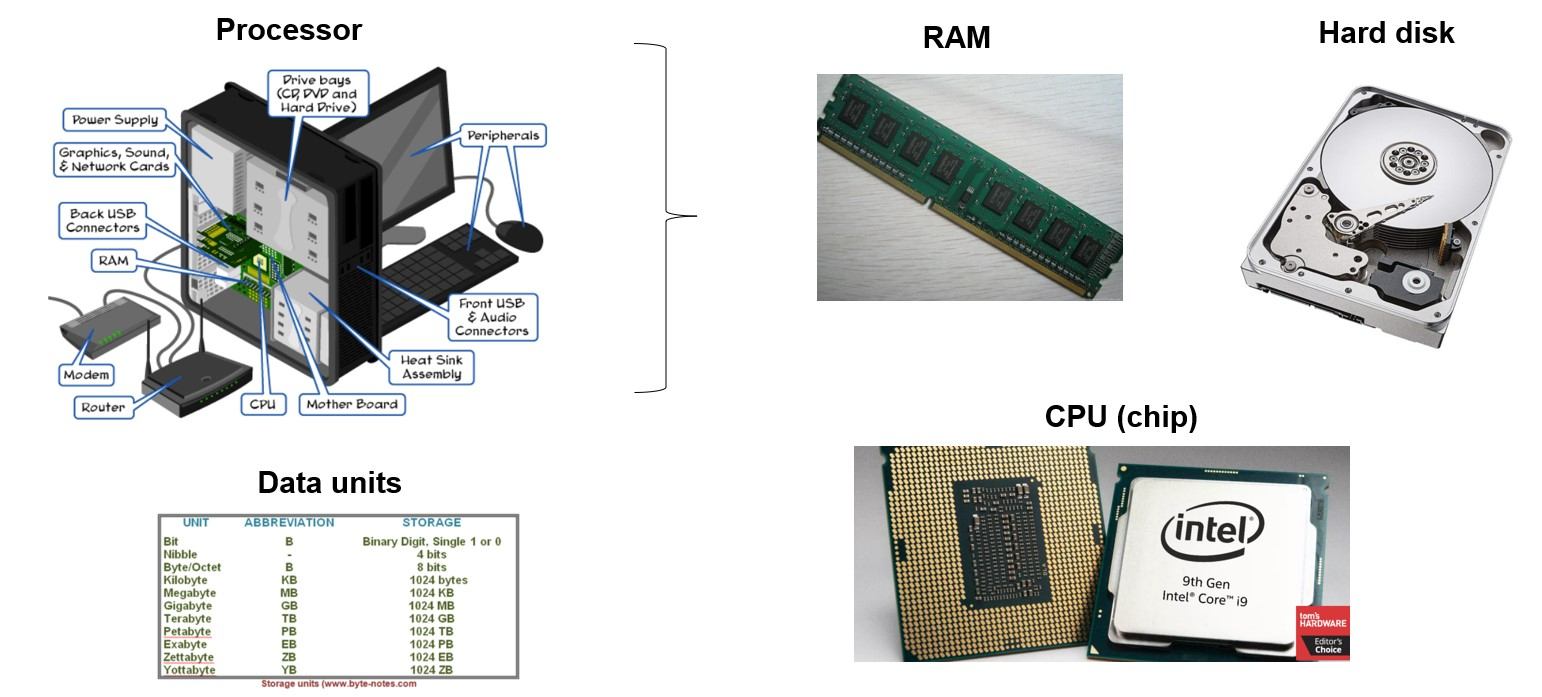
\includegraphics[scale = 0.35]{figures/computer.jpg}
\end{frame}

\begin{frame}
    \frametitle{Operating systems}
    \centering
    
\includegraphics[scale = 0.5]{figures/os.jpg}
\end{frame}

\begin{frame}
    \frametitle{Folder structure}
    \centering
    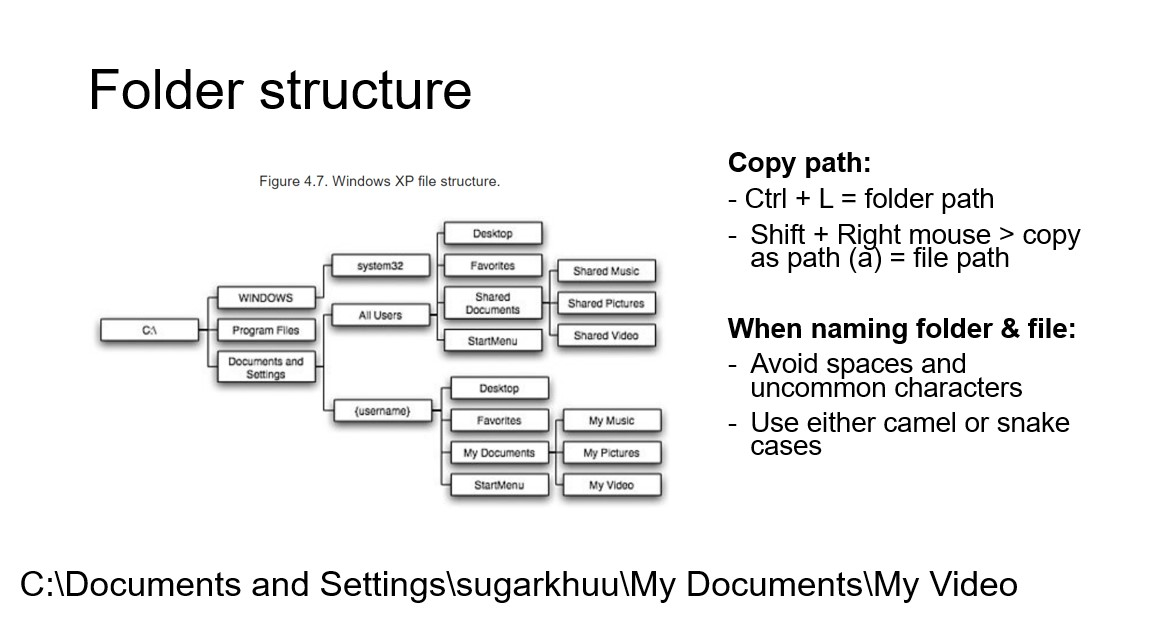
\includegraphics[scale = 0.5]{figures/folder.jpg}
\end{frame}


\begin{frame}
    \frametitle{Command line interpreters/Shells}
    \centering
    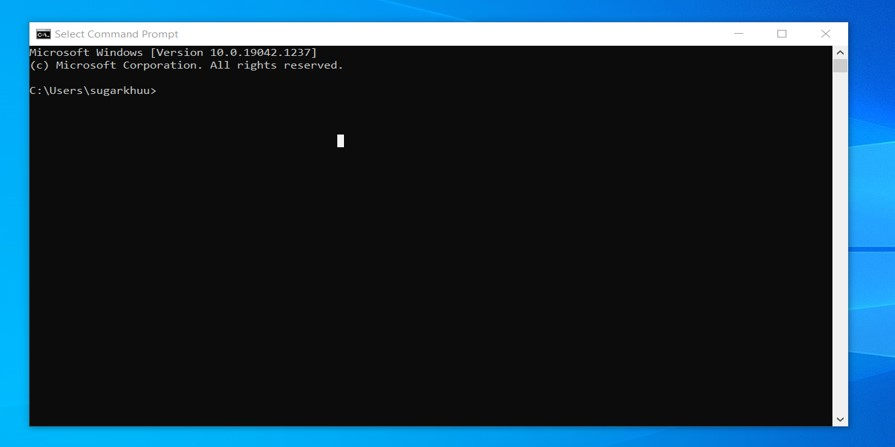
\includegraphics[scale = 0.3]{figures/bash.jpg}

    You are able to control your computer through commanding
    the OS from terminals (Win+CMD, Ctrl+T). More powerful and flexible than usual GUI way of doing things \\

    \begin{itemize}
        \item Windows: Command prompt, Powershell. More recently, Windows Terminal \\
        \item Linux: Bash
        \item Mac: Terminal (zsh)
    \end{itemize}
\end{frame}

\begin{frame}
    \frametitle{Path (environment variable)}
    \centering
    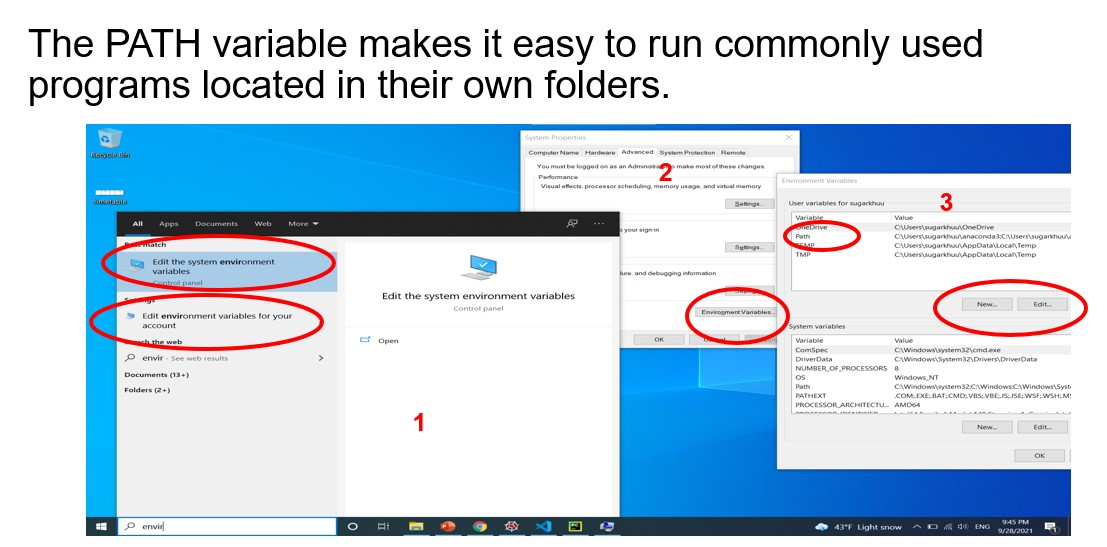
\includegraphics[scale = 0.5]{figures/path.jpg}
\end{frame}

\begin{frame}
    \frametitle{Common CMD/Bash commands}
    \begin{itemize}
        \item cd [cd] – change directory. /? - help
        \item dir [ls] – directory content
        \item copy [cp] – copy file
        \item ren [mv] – rename file
        \item del [rm] – delete file
        \item mkdir [mkdir] – create new folder
        \item exit [exit] - close terminal
        \item cls [ctrl+L] – clear terminal
    \end{itemize}
\end{frame}


%------------------------------------------------
\section{Python} 
% \frame{\tableofcontents[currentsection]}
%------------------------------------------------

\begin{frame}
    \frametitle{Getting Python}
    \centering
    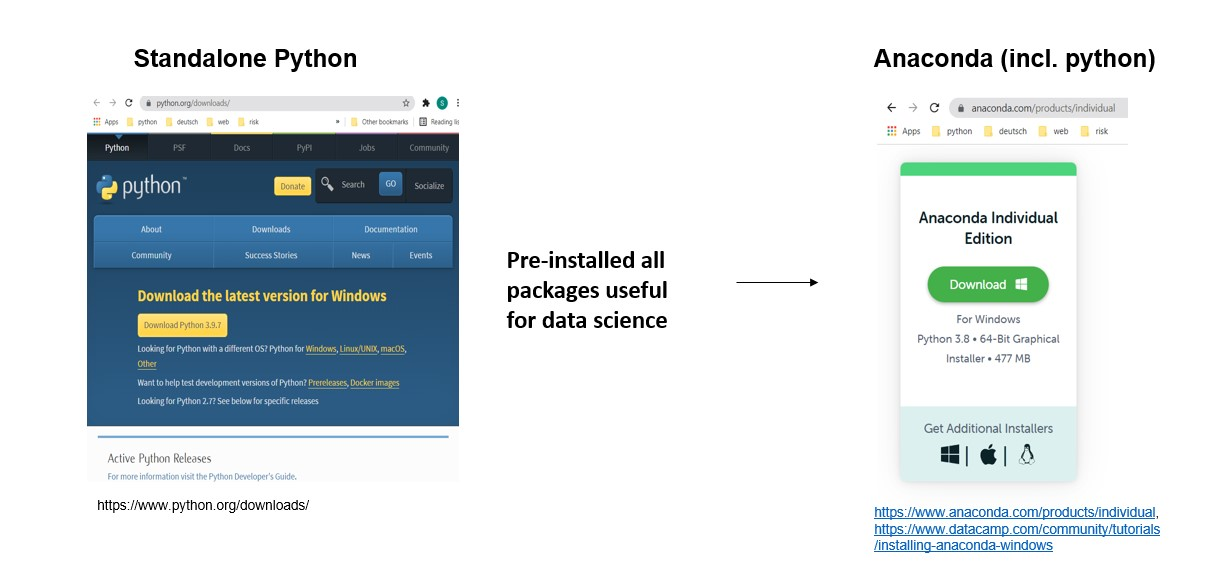
\includegraphics[scale = 0.35]{figures/getpython.jpg}
\end{frame}

\begin{frame}
    \frametitle{What is a programming language?}
    A programming language is a formal language comprising a set of strings 
    that produce various kinds of machine code output.
    Wikipedia \\
    \centering
    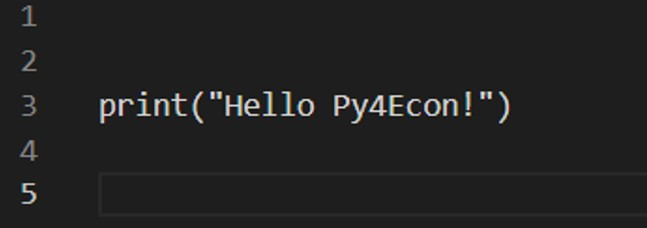
\includegraphics[scale = 0.3]{figures/hello.jpg}   
\end{frame}

\begin{frame}
    \frametitle{Python basic concepts for today:}

    \begin{itemize}
        \item Basic syntax
        \item Basic operators
        \item Packages (+ pip) % pip numpy, pandas # show git examples
    \end{itemize}
\end{frame}


%------------------------------------------------
\section{Code editor} 
% \frame{\tableofcontents[currentsection]}
%------------------------------------------------

\begin{frame}
    \frametitle{Possible to use Python in many environments}

    \begin{enumerate}
        \item Terminal
        \item IDEs – Spyder or Pycharm (IntelliJ), VScode
        \item Notebook -  (\href{https://github.com/susanli2016/Machine-Learning-with-Python}
        {Jupyter notebook})
    \end{enumerate}
\end{frame}

\begin{frame}
    \frametitle{Using VS code (code editor) for Python}
    \centering
    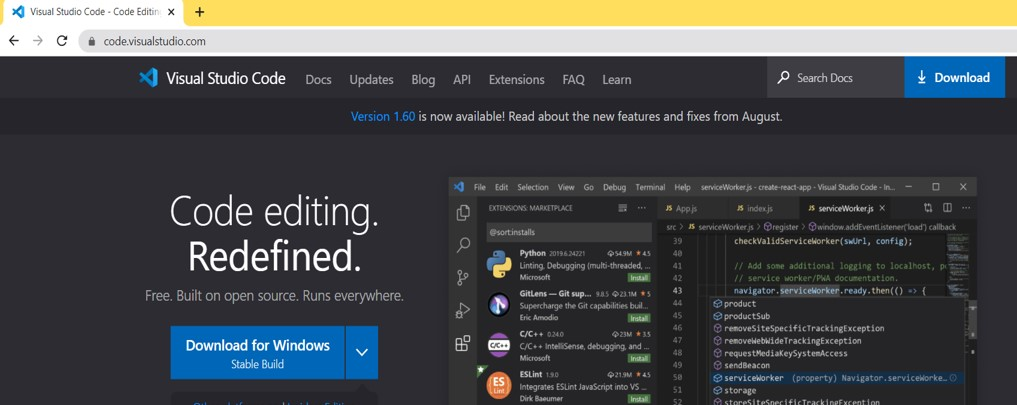
\includegraphics[scale = 0.5]{figures/vscode.jpg}
\end{frame}

%------------------------------------------------
\section{Git/Github} 
% \frame{\tableofcontents[currentsection]}
%------------------------------------------------    


\begin{frame}
    \frametitle{Git – Version control system (VCS)}
    \centering
    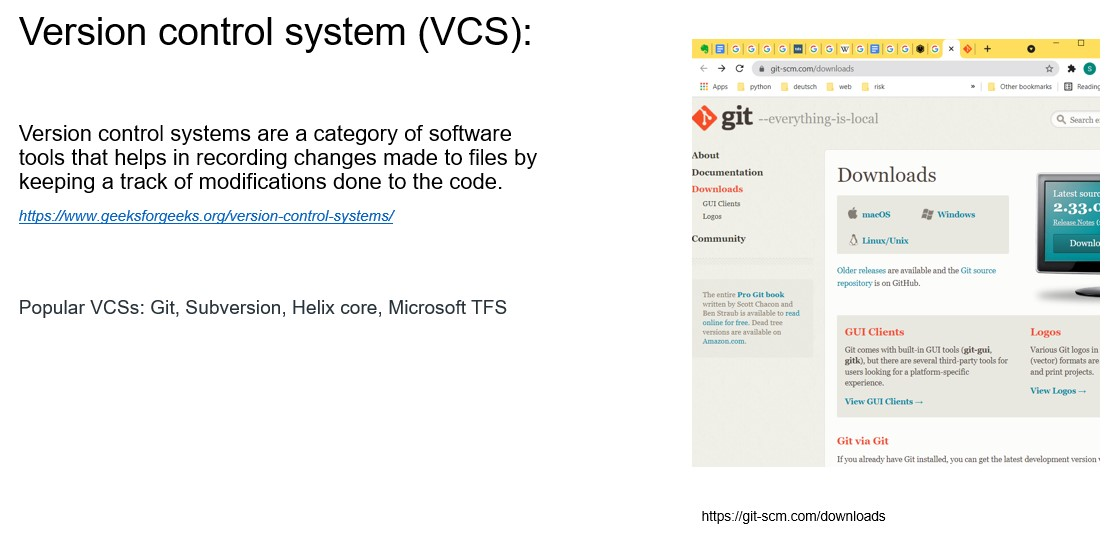
\includegraphics[scale = 0.35]{figures/git.jpg}
\end{frame}

\begin{frame}
    \frametitle{Git – Version control system (VCS)}
    \centering
    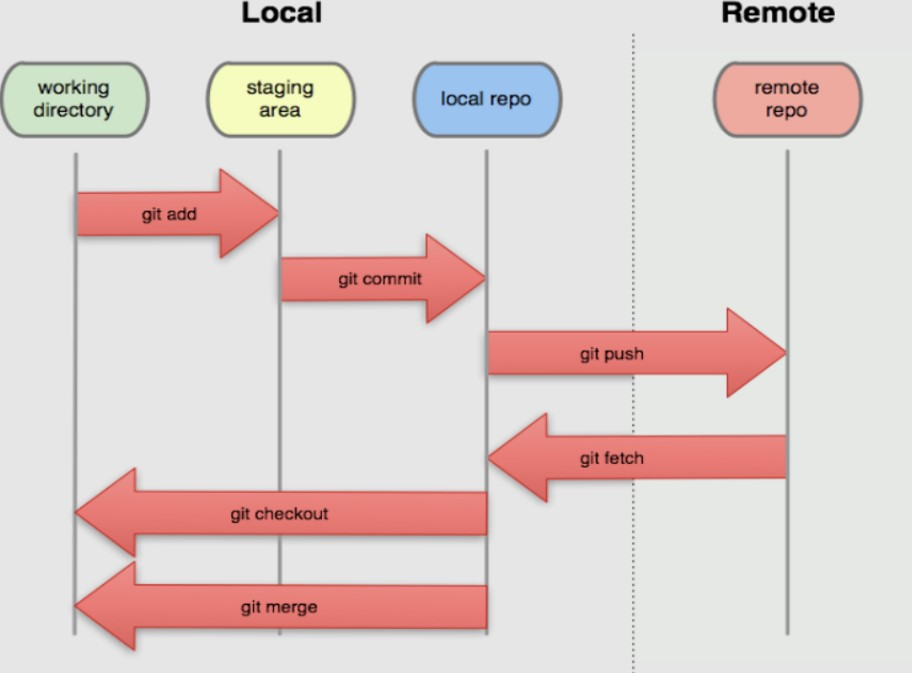
\includegraphics[scale = 0.5]{figures/git_flow.jpg}
\end{frame}

\begin{frame}
    \frametitle{Github – Share everything you want}
    \centering
    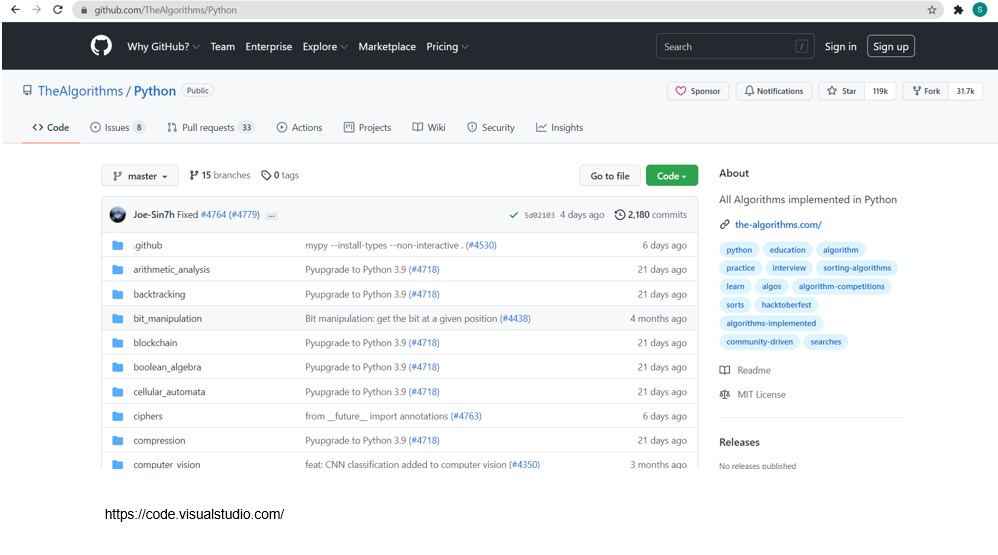
\includegraphics[scale = 0.5]{figures/github.jpg}
\end{frame}

\begin{frame}
    \frametitle{Git bash (terminal)}
    A unix based commands on Windows (Emulator)
    \centering
    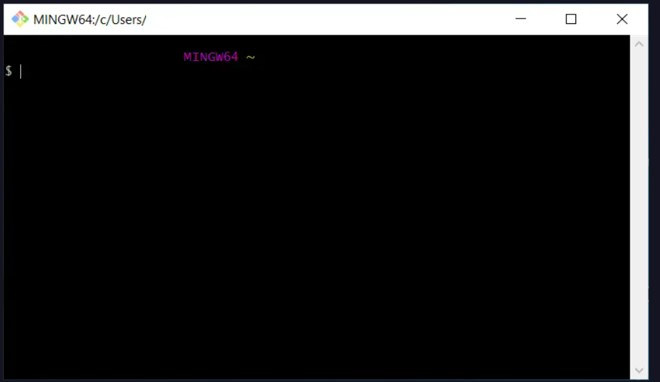
\includegraphics[scale = 0.5]{figures/git_bash.jpg}
\end{frame}


\section{Homework} 

\begin{frame}
    \frametitle{Homework}
    \begin{enumerate}
        \item Task 1
        \item Task 2
    \end{enumerate}
\vskip 2mm
    \begin{itemize}
        \item Submit your result in a "Homework" github repo
        \item Deadline: 1 week%15 January, 2022
    \end{itemize}

\end{frame}

\begin{frame}
    \frametitle{Task 1}
    \begin{enumerate}
        \item Create a new repository in your Github
        \item Clone this repository to your local machine
        \item Create a python file in the local repo (in your folder)
        \item In the file, write a code which asks a question and 
        receives the answer from the user
        \item Commit and push your change
        \item Create 3 more questions, and commit and push
    \end{enumerate}
\end{frame}

\begin{frame}
    \frametitle{Task 2}
    \begin{enumerate}
        \item Нэг компьютерт хоёр үйлдлийн систем суулгаж болох уу?
        \item Path-д программаа оруулаагүй бол яах вэ?
        \item Фолдерийн нэр нь дундаа зайтай байвал фолдерийг танихад ямар асуудал үүсэх вэ?
        \item Git, Github хоёрын ялгаа юу вэ?
        \item Commit, push хоёрын ялгаа юу вэ?
        \item Push хийхээс өмнө олон дахин commit хийж болох уу?
        \item Commit хийхэд github repo-д access хэрэгтэй юу?
    \end{enumerate}
\end{frame}

\begin{frame}
\Huge{\centerline{Thank you!}}
\end{frame}

%----------------------------------------------------------------------------------------

\end{document} 